\documentclass[12pt]{article}
\usepackage{amsmath}
\usepackage{fullpage}
\usepackage{arev}
\usepackage[utf8]{inputenc}
\usepackage[T1]{fontenc}
\usepackage{braket}
\usepackage{bytefield}
\usepackage{qcircuit}

\usepackage{minted}
\usepackage{mdframed}
\usepackage{mathtools}
\usepackage[colorlinks=true,allcolors=black]{hyperref}
%\usepackage{authblk}

\surroundwithmdframed{minted}

\newminted[quil]{text}{fontsize=\footnotesize}
\newminted[python]{python}{fontsize=\footnotesize}
\newminted[bash]{bash}{fontsize=\footnotesize}


\newcommand{\RR}{\ensuremath{\mathbb{R}}}
\newcommand{\CC}{\ensuremath{\mathbb{C}}}
\DeclareMathOperator{\Span}{span}
\DeclareMathOperator{\re}{Re}
\DeclareMathOperator{\im}{Im}
\DeclareMathOperator{\image}{image}
\DeclareMathOperator{\Run}{\mathcal{R}}

\newcommand{\Zero}{\ensuremath{\ket{0}}}
\newcommand{\One}{\ensuremath{\ket{1}}}

\newcommand{\RX}{\ensuremath{\mathtt{RX}}}
\newcommand{\RY}{\ensuremath{\mathtt{RY}}}
\newcommand{\RZ}{\ensuremath{\mathtt{RZ}}}
\newcommand{\CZ}{\ensuremath{\mathtt{CZ}}}
\newcommand{\TGate}{\ensuremath{\RZ(\tfrac{\pi}{4})}}
\newcommand{\TdGate}{\ensuremath{\RZ(-\tfrac{\pi}{4})}}
\newcommand{\CNOT}{\ensuremath{\mathtt{CNOT}}}
\newcommand{\SWAP}{\ensuremath{\mathtt{SWAP}}}
\newcommand{\Hadamard}{\ensuremath{\mathtt{H}}}
\newcommand{\PauliX}{\ensuremath{\mathtt{X}}}
\newcommand{\PauliY}{\ensuremath{\mathtt{Y}}}
\newcommand{\PauliZ}{\ensuremath{\mathtt{Z}}}
\newcommand{\Halt}{\ensuremath{\mathtt{HALT}}}

\title{CS239 Lecture Notes (Week 6)}
\author{%
Robert S.\ Smith\footnote{email: \href{mailto:robert@rigetti.com}{\texttt{robert@rigetti.com}} (corresponding author)} \and
Mark G.\ Skilbeck\footnote{email: \href{mailto:mark.skilbeck@rigetti.com}{\texttt{mark.skilbeck@rigetti.com}}}%
}
\date{}

\begin{document}

\maketitle

\begin{center}
\textit{These are notes for the 6 May 2019 lecture for UCLA's CS239 course. Questions, corrections, and comments are welcome!}
\end{center}

\tableofcontents

% Robert's section
\section{Introduction}

Rigetti is a company in Berkeley, California that manufactures and deploys quantum computers. It is a full-stack company, in that it engages in everything from the fabrication of superconducting qubits on silicon wafers, all the way up to the development of quantum algorithms. We have our own facility for fabricating quantum processors in Fremont, and then we have a couple facilities in Berkeley where we assemble, test, deploy, and maintain these machines.

These quantum computers are real, and accessible today. They are accessed through a product
called Quantum Cloud Services (QCS), which gives users full, exclusive access to these machines.
With that said, quantum computers are also not yet taking over the world. The phone in
your pocket is still more powerful than our deployed quantum processors, but they are getting
better at an ever increasing pace.

It's my understanding that this course will provide each of you a chance to try running some
programs on our quantum processors, and Mark and I are here to tell you how to do that.
For better or worse, we are not salespeople, but engineers who help build this system. We
specialize in the programming of the machine, and we would like to tell you how we think
about wielding it as a computational resource in your arsenal.

We are going to start off by talking about a programming model for quantum software.
Fortunately, it is pretty simple, as we'll see. Next, we'll discuss how this programming
model maps to real quantum computers, which requires unpacking the idea of ``compilation''
a little bit. And lastly, Mark will take the driver's seat and show us how to do quantum
software engineering with the Forest software development kit, using pyQuil in particular.

\section{The Quantum Abstract Machine}
Fundamentally, quantum computers are driven by a physical process. For instance, for
superconducting qubits, one effects change by firing microwave pulses at microscopic
circuits. Each pulse can be seen as a discrete change in the system. Quantum computing
systems of course have other elements to them, like a classical processor to drive the
whole apparatus. Since all of this corresponds to the physical reality of the machine,
we find it prudent to provide an abstract model of this for study. This model is called
the quantum abstract machine, and was defined in its first form in \cite{quilpaper}.

Formally, a quantum abstract machine---or QAM---has six parts:
\begin{description}
\item[Quantum State $\ket{\Psi}$] A quantum state of some number of qubits.
\item[Classical State $C$] A classical state of some number of bits. Chunks of classical memory are usually given names, like $\mathtt{ro}$ for a register of read-out bits. We'll talk about this more later.
\item[Gates $G$, $G'$] A fixed set of static gates $G$, and a fixed set of parametric gates $G'$. The Hadamard gate $\texttt{H}$ is an example of a fixed gate, and $\mathtt{RX}(\theta)$ is an example of a parametric gate.
\item[Program $P$] A program, which is a fixed sequence of instructions. These instructions have a special syntax, called Quil, which we will discuss later.
\item[Program Counter $\kappa$] A program counter, which tells us which instruction to execute next in the program.
\end{description}

Together, these form a six-tuple $(\ket{\Psi}, C, G, G', P, \kappa)$ and it represents the state of a QAM. The QAM can be segmented into three parts:
\begin{itemize}
\item The \emph{state} part, which is $(\ket{\Psi}, C, \kappa)$. These are the bits that change throughout the execution of the program.
\item The \emph{instruction set architecture} or \emph{ISA}, which is $(G, G')$. These dictate both the structure \emph{and} the quantum operations of the machine.
\item The \emph{program}, which is just $P$. We will sometimes write out the instructions of the program in angle brackets. For example, a program that executes an $\PauliX$--gate on qubit $3$ and a $\PauliZ$--gate on qubit $2$ would be written $\langle\PauliX_3,\PauliZ_2,\Halt{}\rangle$.
\end{itemize}
As the program is run instruction-by-instruction, the state changes. For example, if $\PauliX_3$---an X--gate on qubit $3$---is a part of $G$, then that instruction will invoke a transition
\begin{displaymath}
(\ket{\Psi}, C, \kappa) \to (\PauliX_0\ket{\Psi}, C, \kappa+1).
\end{displaymath}
In this case, our quantum state changed, and our program counter bumped up by one. Other instructions affect other parts of the state, sometimes all three, as with measurement.

This model of thinking about computation---the idea of a series of discrete state transitions---is very reminiscent of the Turing machine, and constitutes a so-called \emph{operational understanding} of quantum computation. As such, it's the foundation for how we think about programming the machine. Operational semantics give a very direct intuition for how programs are written and run, but operational semantics sometimes makes it difficult to prove theorems of interest to programming language theorists. That's okay though, since it's possible and in fact not too hard to develop a correspondence between an operational semantics and something else like denotational semantics.

As a matter of vocabulary, a QAM that's simulated by a classical processor is called a \emph{quantum virtual machine} or \emph{QVM}. A QAM that's simulated by a quantum processor is called a \emph{quantum processing unit} or \emph{QPU}.

Anyway, let's go into each element of the QAM with a little bit more detail.

\subsection{The Quantum State}
The quantum state $\ket{\Psi}$ represents the state of the qubits in a QAM. I won't review \emph{all} of the details of the quantum state, which surely has been drilled into your heads by now, but I will make a few salient points, especially in terms of conventions.

The distinguished states of the $k$\textsuperscript{th} qubit are written $\Zero_k$ and $\One_k$. We write the little subscripts because they are in fact distinguished in a physical sense: A physical qubit $5$ doesn't have precisely the same excited state energy as that of another physical qubit, say qubit $7$. Put plainly, $\ket{1}_5\neq\ket{1}_7$.

In isolation, the $k$\textsuperscript{th} qubit occupies a two-dimensional complex Hilbert space, written 
\begin{equation*}
    B_k := \Span_{\CC}\{\Zero_k,\One_k\}.
\end{equation*}
When the qubits interact, the states occupy a larger Hilbert space. For $n$ qubits, we write
\begin{equation*}
    H := \sideset{}{'}\bigotimes_{k=0}^{n-1} B_i = B_{n-1} \otimes B_{n-2} \otimes \cdots \otimes B_1 \otimes B_0.
\end{equation*}
We write $\sideset{}{'}\bigotimes$ with a prime to indicate the tensor product is built on the left. The reason for this is so that we have a nice way to write out the computational basis. Notice how much of a pain it is to write out this basis element of five qubits:
\begin{displaymath}
\Zero_4 \otimes \One_3 \otimes \Zero_2 \otimes \Zero_1 \otimes \Zero_0.
\end{displaymath}
It's much easier to write $\ket{01000}$. Even better, if we write out the basis elements in lexicographic order
\begin{displaymath}
\ket{00000}, \ket{00001}, \ket{00010}, \ldots, \ket{11110}, \ket{11111};
\end{displaymath}
then the $k$\textsuperscript{th} element corresponds to the binary expansion of $k$. In fact, the state
\begin{displaymath}
\alpha_0\ket{00000} + \alpha_1\ket{00001} + \cdots + \alpha_{30}\ket{11110} + \alpha_{31}\ket{11111}
\end{displaymath}
is stored in a classical computer exactly as an array of complex numbers, as seen in fig.~\ref{fig:fiveq}.

\begin{figure}
    \centering
    \begin{bytefield}{5}
        \wordbox{1}{$\re \alpha_0$} & \wordbox{1}{$\im \alpha_0$}
        & \wordbox{1}{$\re \alpha_1$} & \wordbox{1}{$\im \alpha_1$}
        & \wordbox{1}{$\cdots$}
        & \wordbox{1}{$\re \alpha_{31}$} & \wordbox{1}{$\im \alpha_{31}$}
    \end{bytefield}
    \caption{A $5$-qubit quantum state stored as an array. The real and imaginary parts are typically stored as 64-bit double-precision floats.}
    \label{fig:fiveq}
\end{figure}

Gates also follow this ordering convention. The \CNOT{} gate acting on qubits $0$ and $1$, namely
\begin{displaymath}
\CNOT_{01} : B_1 \otimes B_0 \to B_1 \otimes B_0
\end{displaymath}
has the presentation as a matrix
\begin{displaymath}
\texttt{CNOT}_{01} :=
\begin{pmatrix}
0 & 1 & 0 & 0\\
1 & 0 & 0 & 0\\
0 & 0 & 1 & 0\\
0 & 0 & 0 & 1
\end{pmatrix},
\end{displaymath}
where qubit $1$ is the control qubit, and qubit $0$ is the target qubit. This doesn't look like the normal \CNOT{}-matrix because we've fixed our space and a consequent basis for that space. On the other hand, the operator $\CNOT_{10}$ on the same space has the usual presentation:
\begin{displaymath}
\texttt{CNOT}_{10} :=
\begin{pmatrix}
1 & 0 & 0 & 0\\
0 & 1 & 0 & 0\\
0 & 0 & 0 & 1\\
0 & 0 & 1 & 0
\end{pmatrix}.
\end{displaymath}
You should verify that both of these matrices respect what we mean by $\CNOT{}$ in our convention of space. This whole topic of ordering is delved into in \cite{shouts}.

With all of this, we can write a quantum state $\ket{\Psi}$ of $n$ qubits as
\begin{displaymath}
\ket{\Psi} = \sum_{k=0}^{2^n-1} \alpha_k\ket{k},
\end{displaymath}
where $\ket{k}$ is to be understood as the $k$\textsuperscript{th} computational basis element.

I promise that all of this isn't just mathematical nonsense; it's important for understanding what your programs are doing, and how to precisely read a quantum state as a list of amplitudes. I can't count the number of times folks at Rigetti---myself included---have stumbled in the wrong direction because we didn't have this ordering business sorted out.

There's nothing more to say about states, except that the actual amplitudes of the state aren't typically directly accessible to you as a programmer. We will learn a bit later how we can change this state, with gates like $\texttt{CNOT}_{10}$.

\subsection{Gates and the ISA}
Physical quantum processors have physical constraints. For example, in superconducting qubit systems, if two physical qubits are not near one another, then it's generally not possible for them to interact in a single, discrete operation. So while we might have a quantum computer that supports the \CNOT{} gate, we aren't really being precise by saying that. Instead, we ought to say something like ``our computer supports a \CNOT{} gate between qubits $1$ and $0$, as well as between qubits $2$ and $1$.'' More exotic gates, such as the M{\o}lmer--S{\o}rensen gate\cite{molmer} can operate on more than two qubits simultaneously. This gate has the action of producing something like a GHZ-state:
\begin{displaymath}
\ket{0}^{\otimes n} \mapsto \frac{e^{i\phi_0}\ket{0}^{\otimes n} + e^{i\phi_1}\ket{1}^{\otimes n}}{\sqrt{2}}.
\end{displaymath}

The role of $G$ and $G'$ in the QAM is to define precisely what the machine supports. Because qubits can support operations, qubit pairs can support operations, qubit triplets etc., we formally consider the ISA of a quantum abstract machine to be a \emph{hyper-multigraph}. That is to say, the ISA is a set of vertices $V$ which represent the qubits, and a set of hyperedges containing:
\begin{itemize}
    \item A map $E_1$ from\footnote{The notation $\tbinom S n$ is the set of $n$-element subsets of $S$.} $\tbinom V 1 = V$ to a set of single-qubit gates,
    \item A map $E_2$ from $\tbinom V 2$ to a set of two-qubit gates,
    \item A map $E_3$ from $\tbinom V 3$ to a set of three-qubit gates,
\end{itemize}
and so on up to a map $E_n$ from $\tbinom V {\vert V\vert} = \{V\}$ to a set of $\vert V\vert$-qubit gates. We call $E_i$ a \emph{hyperedge of valence $i$}. As shorthand, we might write this graph as \[\left(V,\{E_1,\ldots,E_{\vert V\vert}\}\right).\] For superconducting qubits, the valence is usually limited to $2$, that is, we have both one- and two-qubit gates\footnote{This isn't strictly true for superconducting qubits, and is certainly not true for other qubit technologies like ion traps.}.

The hyper-multigraph presentation of an ISA is useful for understanding at a glance what a quantum abstract machine can do, because it makes for drawing nice pictures\footnote{Sometimes we talk about the \emph{qubit graph}, which is a traditional graph whose vertices are qubits and whose edges represent the existence of \emph{any} two-qubit gate between them.}, but it's often useful to just bag everything together. In fact,
\begin{equation}
    G \cup G' = \bigcup_{i=1}^{\vert V\vert} \image E_i.
\end{equation}
The set $G$ is specifically the set of \emph{static gates}, linear operators $H\to H$. These often include the usual suspects, like Pauli gates, Hadamard, etc. The set $G'$ is specifically the set of parametric gates, families of linear operators parameterized by a set of real numbers. These often include rotation gates and $\mathtt{CPHASE}$.

What's important to note---in the context of the specification of a QAM's ISA---is that there is no ``ordained'' \CNOT{} gate. There are only \CNOT{} gates that act on vertices of the qubit graph.

\subsection{Classical Memory and Measurement}

Formally, the classical memory $C$ is just a tuple of bits. This is very nice mathematically, but cumbersome as a programmer. As such, we can provide structure to $C$ by declaring memory. Memory can be partitioned into bits, octets, signed integers, and (approximations of!) real numbers. We can give such memory name using \verb|DECLARE| syntax.

\begin{quil}
DECLARE ro BIT[8]
DECLARE mem OCTET[32]
DECLARE theta REAL
DECLARE count INTEGER
\end{quil}

This is a syntax for outlining the structure of a memory $C$ of $8+8\cdot 32+64+64=392$ bits, and we can always formalize it by way of a \emph{memory map}. For instance, suppose $C\in\{0,1\}^{392}$. If both \verb|INTEGER| and \verb|REAL| are 64-bits, then we might have the memory map:
\begin{itemize}
    \item $\texttt{ro}[i] = C_i$ for $0 \leq i < 8$,
    \item $\texttt{mem}[i] = (C_{8i+8}, C_{8i+9}, \ldots, C_{8i+15})$ for $0\leq i < 32$,
    \item $\texttt{theta} = (C_{264}, C_{265}, \ldots, C_{327})$, and
    \item $\texttt{count} = (C_{328}, C_{329}, \ldots, C_{391})$.
\end{itemize}

From a formal perspective, this naming business isn't necessary. (That's why the QAM just has a $C$.) However, as a programmer, it's useful.

Measurement is one kind of instruction in the QAM that affects both the quantum state and classical state, since the result of the measurement is stored. As quantum mechanics prescribes, it's non-deterministic. Suppose we perform a measurement on qubit $k$ and opt to store the resulting bit at $C_j$. This induces a projection $\pi\in\big\{\ket{0}_k\bra{0}_k,\ket{1}_k\bra{1}_k\big\}$ along with the storage of a bit $b\in\{0,1\}$. Our QAM's state transitions non-deterministically as
\begin{displaymath}
(\ket{\Psi}, C, \kappa) \to \left(\frac{\pi\ket{\Psi}}{\Vert\pi\ket{\Psi}\Vert}, C[C_j:=b], \kappa+1\right).
\end{displaymath}
When writing out the formal semantics of the QAM, the non-determinism is often expressed in terms of a more general concept called density operators, which I won't get into.

In Quil syntax, the instruction is written \[\texttt{MEASURE~$k$~$C_j$}.\] We will look into more Quil syntax next.

\subsection{Quil: A Quantum Instruction Language}
We've talked an awful lot about the structure of a quantum abstract machine and what you can do with it, but we've only written down mathematical descriptions of these things, and not talked about a way to write concrete \emph{programs}. The purpose of Quil is to describe our program $P$---a sequence of state transitions of the QAM---with a concrete syntax. The syntax looks a lot like assembly, but is slightly higher level than that. The ``hello world'' of quantum computing is the construction and measurement of a Bell state. This is written:
\begin{quil}
DECLARE ro BIT[2]      # declare the existence of a 2-bit register in C
H       0              # Hadamard on qubit 0
CNOT    0 1            # CNOT with control 0 and target 1
MEASURE 0 ro[0]        # measurement of qubit 0 into the first bit of ro
MEASURE 1 ro[1]        # measurement of qubit 1 into the second bit of ro
\end{quil}

The whitespace is irrelevant, of course. As can be seen, excepting the \verb|DECLARE| directive, each line is an instruction. The instructions are precisely the elements of the sequence $P$. We would say this Quil code is \emph{native} on a QAM with $\{\Hadamard_0, \CNOT_{01}\}\subset G$.

We can invoke parametric gates with syntax that you would expect:
\begin{quil}
DECLARE theta REAL
RX(pi/2) 0
RZ(theta) 1
\end{quil}

There's a host of standard gates, most of them with the familiar names: \verb|X|, \verb|H|, \verb|CNOT|, etc. But we can define new gates by writing out their matrix:
\begin{quil}
DEFGATE new-gate:
    0, 1, 0, 0
    1, 0, 0, 0
    0, 0, 1, 0
    0, 0, 0, 1
\end{quil}
This defines a sort of ``flipped \verb|CNOT|'', with the target and control swapped. We could of course accomplish this with the \verb|SWAP| gate.

Quil has many language features. It contains a host of classical instructions like \verb|MOVE|, \verb|STORE|, and \verb|ADD|, all causing transitions of $C$, but we won't get into those. It also allows for general control flow, including loops and branches with the \verb|JUMP| and \verb|JUMP-WHEN| instructions. These are reasoned about as transitions of $\kappa$ and are very important for certain programs like active reset, but we also will not get into those.

One special instruction, however, is \Halt{}, which is an instruction which does \emph{not} transition $\kappa\to\kappa+1$, in effect, freezing the state of the QAM.

Mark will be speaking a bit later about how to write Quil using our Python library called pyQuil, but I'd like to shift gears a bit and talk about how we can be more expressive as programmers by introducing the notion of compilation.

\section{Compilation}

Compilation of quantum programs serves two critical roles. First, it allows us as programmers express programs with a broader set of primitives, since quantum computers expose only a limited set of operations. Second, compilation provides means for optimizing the program, generally making the program shorter or make use or more efficient operations.

Optimizing compilers for \emph{classical} programs are merely a convenience. An optimized classical program may run in less time or consume less memory. This, in turn, means that I, the programmer, have to wait less, or use a less expensive computer, in order to accomplish the task I set out to do with the classical computer. The optimization (usually) does not affect the correctness or accuracy of the program.

However, in the case of quantum programs, optimization serves a much more important role outside of providing convenience. While a quantum computer is running, it \emph{decoheres} due to natural effects, which causes the machine to produce incorrect results with higher probability over time. For superconducting qubit processors, there's an associated measure for this decoherence, called the $T_1$ and $T_2$ times. Roughly speaking, these times put a bound on the amount of time a program can run before it produces bad results more than $50\%$ of the time. Currently, $T_1$ times sit around $1$ to $100\,\mu\mathrm{s}$.

I won't delve into the details as to \emph{why} this time limit exists, except to say one of the top areas of research is how to build machines that ever increase this limit. Since the development of the first superconducting qubits, this time has been improved exponentially, for a quantum-Moore's-like law.

Anyway, a compiler has the role of optimizing your program, to potentially take a long program and make it shorter, giving the programmer more freedom and certainty that their program will run as best it can.

\subsection{The Problem of Compilation}

With the QAM formalism in hand, we can state the problem of compilation quite simply. First, let's introduce a function $\Run$ which takes a QAM and runs the program, producing a final QAM if the program has halted. For instance,
\begin{displaymath}
\Run (\Zero, \mathtt{0}, \{\PauliX_0\}, \emptyset, \langle \PauliX_0, \Halt\rangle, 0)
=
(\One, \mathtt{0}, \{\PauliX_0\}, \emptyset, \langle \PauliX_0,\Halt\rangle, 1).
\end{displaymath}
It of course may not be the case that a program terminates, in which case, the function $\Run$ isn't well defined.

With this, it is easy to state the compilation problem:
\begin{framed}
\noindent \textbf{Compilation problem in plain English:} Given a QAM and a target gate set $(G, G')$, find a QAM with that gate set, and running the QAMs to completion gives equivalent classical and quantum states.
\end{framed}
\noindent A more mathematical statement would be:
\begin{framed}
\noindent \textbf{Compilation problem in mathematicians' English:} Let \[M_{\textrm{src}} := (\ket{\Psi}, C, G_{\textrm{src}}, G'_{\textrm{src}}, P_{\textrm{src}}, \kappa)\] and \[M_{\textrm{target}} := (\ket{\Psi}, C, G_{\textrm{target}}, G'_{\textrm{target}}, x, \kappa)\] both be QAMs. Also let
\begin{displaymath}
M^*_{\textrm{src}} := \Run M_{\textrm{src}}\qquad\text{and}\qquad
M^*_{\textrm{target}} := \Run M_{\textrm{target}}
\end{displaymath}
whose quantum states are $\ket{\Psi^*_{\textrm{src}}}$ and $\ket{\Psi^*_{\textrm{target}}}$ respectively. Then for an arbitrary but fixed $\epsilon>0$, find a program $x$ such that the respective classical states are identical and
\begin{displaymath}
\left\Vert\ket{\Psi^*_{\textrm{src}}} - \ket{\Psi^*_{\textrm{target}}}\right\Vert < \epsilon.
\end{displaymath}
\end{framed}

We might ask, is such an $x$ guaranteed to exist? Except in a small number of pathological cases, the answer is a resounding ``yes'', provided $M_{\textrm{src}}$ and $M_{\textrm{target}}$ are universal. In fact, provided the source and target QAMs have hyperedges of equal valence, the size of $x$ will grow as $(\log (1/\epsilon))^{3.9}$. This is a truly remarkable result known as the Solovay--Kitaev theorem.

If we are to solve the compilation problem, what is involved exactly? There are a lot of approaches to compilation, but we will discuss three frequent tasks: decomposition, routing, and optimization.

\subsection{Decomposition}
In essence, \emph{all} compilation problems are decomposition problems; we wish to express objects in one semantic domain as objects with equivalent properties in another semantic domain. However, here, we mean something more specific. Returning back to the hyper-multigraph view of a QAM, it might be that our source QAM has hyperedges whose valence is larger than any of those in the target QAM. For instance, we might write a program which uses the Toffoli gate \[\textrm{CCNOT} := (I \otimes I) \oplus \CNOT{}\] whose valence is $3$, but our target QAM only has one- and two-qubit gates. The goal of decomposition is to re-express our high-valence gates in terms of products of gates whose valences match the target gate set. This isn't any sort of \emph{mathematical} requirement, but it makes solving the compilation problem a bit more principled.

Fig.~\ref{fig:ccnot} shows an example decomposition of $\mathtt{CCNOT}_{012}$ into the set
\begin{displaymath}
\{\CZ_{\{01,02,12\}}, \RX(\pm\pi/2)_{\{0,1,2\}},\RZ(\pm\pi/4)_{\{0,1,2\}} \}.
\end{displaymath}
Note the all-to-all connectivity of the qubits.
\begin{figure}[h]
  \centering
  \hspace{0.3cm}
  \Qcircuit @C=0.6em {
    %%%%%%
    & \control \qw & \qw & {}  & {} & \qw & \qw & \qw
    & \control \qw & \qw &
    \qw & \qw & \control \qw & \qw & \control \qw & \gate{\TGate} &
    \control \qw & \qw \\
    %%%%%%
    & \control \qw \qwx & \qw & {=} & & \qw & \control \qw & \qw &
    \qw \qwx & \qw & \control \qw & \qw & \qw \qwx &
    \gate{\TGate} & \targ \qwx & \gate{\TdGate} & \targ \qwx  & \qw \\
    %%%%%%
    & \targ \qw \qwx & \qw & {} & {} & \gate{H} & \targ \qwx &
    \gate{\TdGate} & \targ \qwx & \gate{\TGate} & \targ \qwx &
    \gate{\TdGate} & \targ \qwx & \gate{\TGate} & \gate{H} & \qw & \qw & \qw }
  \caption{A decomposition of $\mathtt{CCNOT}$ into six \CNOT{} gates \cite{shende}.}
  \label{fig:ccnot}
\end{figure}

Using this identity allows us to reduce just $\mathtt{CCNOT}$, but there are algorithms to decompose gates of general valence, including one from Solovay and Kitaev\cite{skalg}. These algorithms usually come at a great cost, however. In general, edges of high valence decompose into an exponential number of one- and two-qubit operators.

Provided we've used a collection of identities and decomposition methods, we still aren't in a form which will generally respect a QAM of interest. We do have a program whose gates have the right target valences, but they're perhaps not gates that are available to us. This leads to the next problem of quantum compilation.

\subsection{Routing}
Given a program in a QAM with all-to-all connectivity, we wish to compile the program so it conforms to the given connectivity. This problem is relatively simple when the program has gates whose matrices are found in the edges---for one can often use a chain\footnote{More specfically, if one is compiling an operator $U_{pq}$ where there is no $p$--$q$ edge, then one can perform a series of $\SWAP{}$s on qubits $p$ and $q$ so that $U$ in effect operates on an edge that \emph{does} exist.} of \SWAP{} gates---but more difficult when they're not. Suppose our gate set of our target QAM is
\begin{displaymath}
G\cup G' = \{ \RX(\pm\pi/2)_{\{0,1,2\}}, \RZ(\theta)_{\{0,1,2\}}, \CNOT_{\{01, 12\}} \}.
\end{displaymath}
In our Toffoli gate example, there are two $\CNOT_{02}$ gates that need to be routed, and a couple Hadamard gates that need to be converted. The Hadamard gates are easy in this case:
\begin{equation*}
\Hadamard = \RZ(\pi/2)\RX(\pi/2)\RZ(\pi/2).
\end{equation*}
This formula needn't be seen as magic; it can be understood in general as an Euler decomposition, as with rotations in $\mathrm{SO}(3)$. Routing the \CNOT{} gate is also quite simple, though for different reasons, with the identity:
\begin{equation*}
    \CNOT_{02}=\CNOT_{12}\CNOT_{01}\CNOT_{12}\CNOT_{01}.
\end{equation*}
This identity can be used recursively for a longer-range \CNOT{}s.
All of these identities, expansions, \SWAP{} gates, etc.\ usually lead to redundant and inefficient code. This is where optimization is helpful.

\subsection{Optimization}
There are many optimization techniques for quantum programs. We will just mention a few:
\begin{itemize}
    \item Allocating qubits so that gates run more favorably, due to either their connectivity to neighboring qubits, or due to the qubits' physical performance characteristics\cite{noisycomp}.
    \item Collecting groups of instructions and searching for simple reducing identities, such as $\Hadamard \Hadamard=\mathtt{I}$, $\RX(\alpha)\RX(\beta)=\RX(\alpha+\beta)$, and the like.
    \item Taking advantage of known quantum state preparations, so that e.g. when an operator is acting on an eigenstate, that operator can be eliminated, as with $Z$ and the $\Zero$ state.
\end{itemize}

Industrial-strength quantum optimizing compilers, such as quilc, contain all of these methods and more, arranged cleverly so that you can convert just about any QAM into a large collection of other QAMs, including all currently known superconducting architectures.

\section{Programs Below Quil}

I want to end my section by talking a little bit about what happens to Quil code when it's about to be run. As I said earlier, Quil isn't \emph{quite} an assembly language, even if it's written for the ISA of the physical device. As such, there's one more level of compilation that's very close to traditional assembling.

Superconducting qubits, at the end of the day, operate off of microwave pulses and currents. So any code written needs to turn into a sequence of pulse-firings or current-drives. These are controlled by a plurality of processors which can---and do---operate on the QPU in parallel.

The waveforms are generally not as sophisticated as one might think. An $\RX(\pi/2)$ gate corresponds to a waveform that looks something like $\sin(\omega t)e^{t^2}$, where $\omega$ is a frequency in the 5~GHz range. The Quil code
\begin{quil}
RX(pi/2) 3
RX(pi/2) 5
\end{quil}
would assemble into two of these sinusoidal pulses that are fired synchronously at qubits $3$ and $5$.

As a rule of thumb, one-qubit gates usually have a duration of around 20 to 50~ns, while two-qubit gates have a duration of around 80 to 200~ns. To me, it is very remarkable that these gates-measured-in-nanoseconds can effect change in a quantum state that cannot be stored on my laptop feasibly.

With that, I would like to hand it over to Mark, who will discuss how to actually use all of these tools to write software.

\newpage

% Mark's section
\section{Quantum Software Engineering with the Forest SDK}

\subsection{The Forest SDK}

\begin{center}
Info: \url{https://rigetti.com/forest}
\end{center}

The Forest SDK provides a powerful and performant library of tools that are useful in the development of quantum algorithms. Foremost it provides: an optimizing compiler (\verb|quilc|); a quantum virtual machine (\verb|qvm|) for prototyping and debugging; and a Python-based interface to the Quantum Cloud Services (QCS) stack. To install the Forest SDK, follow the URL appropriate for your computer:
\begin{itemize}
    \item macOS: \href{https://downloads.rigetti.com/qcs-sdk/forest-sdk.dmg}{\underline{dmg installer}}
    \item Linux-based: \href{https://downloads.rigetti.com/qcs-sdk/forest-sdk-linux-deb.tar.bz2}{\underline{deb installer}} or \href{https://downloads.rigetti.com/qcs-sdk/forest-sdk-linux-barebones.tar.bz2}{\underline{barebones tarball}}
    \item Windows: \href{https://downloads.rigetti.com/qcs-sdk/forest-sdk.msi}{\underline{msi installer}}
\end{itemize}
Finally install pyQuil with either
\begin{bash}
pip install pyquil==2.7.2
\end{bash}
or
\begin{bash}
conda install -c rigetti pyquil==2.7.2
\end{bash}

\subsection{The Quil Compiler}
\begin{center}
Source Code: \url{https://github.com/rigetti/quilc/}
\end{center}

Quantum programs that are intended to be run on Rigetti QPUs are specified in the assembly-like Quil. While Quil is somewhat low-level it provides methods of abstraction. For example, the base language provides you with many of the gates commonly seen in the literature (e.g. \Hadamard{}, \CNOT{}). Quil's \verb|DEFGATE| allows us to define new gates, by providing a name and some unitary matrix. We also frequently find it helpful to think in terms of circuits---collections of gate applications. Quil provides \verb|DEFCIRCUIT| for this case.

It is ultimately expected that our Quil programs will be executed on a QPU. However, the gates that a QPU understands are typically very limited---this small set of supported gates is called the native gateset of the QPU. Rigetti's native gateset includes just three 1Q gates $\RX(\pm\pi/2)$ and $\RZ(\alpha)$ as well as one 2Q gate \CZ{}. (It is an incredible result of quantum computing research that just these three gates can produce any arbitrary unitary gate---they are universal). 

This presents a problem: Quil the language provides gates not in the native gateset, and further it provides ways to create new gates, also not in the native gateset! And all this with the expectation that it can be run on a QPU. We might just require that Quil programs target the native gateset and be done with it, but that's no fun for anyone. Methods of abstraction make for a powerful and expressive language. Instead we offload this overhead to the compiler: we provide quilc with an arbitrary Quil program and some description of the architecture that we want to target called the ISA. (Technically the ISA encompasses more than just the native gateset: we can include information about the topology and specifications of the available qubits.) The compiler then produces Quil code that targets the specified ISA.

Fortunately the compiler isn't tied to just the Rigetti architecture. In fact it has support for various architectures including Google's 72Q ``Bristlecone'' device, and IBM's 16Q ``ibmqx5'' device. These are ISAs that are hard-coded into the compiler, but implementing a new ISA is mostly as simple as writing out a JSON file and giving it to the compiler.

The compiler does an awful lot more than just mechanically translate non-gateset instructions to gateset instructions. It applies numerous optimization routines, determines resource usage amongst instructions, decomposes complex unitary matrices into smaller and smaller square matrices. All with the intent that the resulting program is equivalent to---but more efficient than---the input program.\footnote{There are unfortunate cases where the compiler does a poor job and ends up producing unnecessarily complex programs. But that's good---we have problems to keep us employed.}

After installing \verb|quilc| you can send it input directly through the command line. For example compile a Hadamard gate on qubit zero:
\begin{bash}
echo "H 0" | quilc

RZ(pi/2) 0                  # Entering rewiring: #(0 1 2 3 4 5 6 7)
RX(pi/2) 0
RZ(pi/2) 0
HALT                        # Exiting rewiring: #(0 1 2 3 4 5 6 7)
\end{bash}
As expected, the compiler has translated the non-native gate \verb|H 0| into a sequence of native gates.

If your program is longer, we can separate them with newlines. This requires the \verb|-e| option to \verb|echo|:
\begin{bash}
echo "H 0\nH 1" | quilc

RZ(pi/2) 0                  # Entering rewiring: #(0 1 2 3 4 5 6 7)
RX(pi/2) 0
RZ(pi/2) 0
RZ(pi/2) 1
RX(pi/2) 1
RZ(pi/2) 1
HALT                        # Exiting rewiring: #(0 1 2 3 4 5 6 7)
\end{bash}

If the command line is getting too unweildy, we can write the same program in a file, say \verb|super.quil|:
\begin{quil}
H 0
H 1
\end{quil}
and then we can \verb|cat| this file into the compiler: \verb/cat super.quil | quilc/.

Try the following and reason about the results:
\begin{itemize}
\item Consecutive Hadamards on the same qubit.
\item Two \verb|H| on the same qubit sandwiching a \verb|H| on a different qubit.
\item Two \verb|H| on the same qubit, sandwiching a \verb|CNOT| on the same qubits.
\end{itemize}

See \verb|quilc --help| for options to configure the compiler. What happens if you use \verb|quilc --isa ibmqx5| for the above?

\subsection{The QVM}
\begin{center}
Source Code: \url{http://github.com/rigetti/qvm}
\end{center}

QPUs are a scarce resource. They are expensive. And noisy. And don't have many qubits. Think about the early days of classical computing---those computers, UNIVAC, ENIAC, etc.\ filled rooms. They were programmed with switches or punched cards, and those programs were debugged by the same process many of us write code today---try it and see. Except back then \emph{try it and see} might mean \emph{wait until tomorrow for the results} followed by \emph{explain to your supervisor why you wasted hours of compute time and \$\$\$ because of a misplaced semi-colon}.

QPUs of today are somewhat like those old big goofy computers. But today we have much better technology to support that scarce resource. We have the modern internet and all the cool stuff that it supports, so that we can share QPU resources pretty efficiently over the network. But at a more immediate level, we can retain the feel of rapid prototyping of code by targeting a quantum virtual machine (QVM).

The spooky probabilistic essence of quantum mechanics can be simulated on classical computers. While the results are \emph{not} obtained by truly quantum means, and the classical resource usage does not scale too nicely\footnote{The wavefunction of $n$ qubits is a $2^n$-length array of complex coefficients. The memory required for a 26-qubit simulation is of order 1~GB; for 36 qubits, 1~TB. You see the unfortunate situation.}, the behaviour and evolution of the wavefunction are approximated well-enough. The upshot of the above is that with reasonably powerful computers (laptops will generally do fine for low numbers of qubits, around $26$) we can enjoy the rapid prototype-feedback loop that we take for granted when developing algorithms for classical computers.

To get a feel of the QVM, you can interact with it directly on the command line (as with \verb|quilc|). The QVM takes as input some Quil code, and then will return to you the final state of the wavefunction. For example, let's investigate how \verb|H 0| changes the state of the wavefunction:
\begin{bash}
echo "H 0" | qvm --quiet

Classical memory (low -> high indexes):
    No memory.
Amplitudes:
    |0>: 0.7071067811865475,                                    P= 50.0%
    |1>: 0.7071067811865475,                                    P= 50.0%
\end{bash}
The wavefunction is in an equal superposition of $\ket{0}$ and $\ket{1}$. As with \verb|quilc|, you can use the \verb|-e| option to \verb|echo| or use \verb|cat|.

With the QVM, explore and reason about the wavefunction in the following situations:
\begin{itemize}
    \item Flip a single arbitrary bit in the ket. Flipping the $k$\textsuperscript{th} bit has a state that can be written $\ket{2^k}$. For example, flipping the third bit would be $\ket{2^3}=\ket{1000}$.
    \item Construct a Bell state: $\tfrac{1}{\sqrt{2}}(\ket{00}+\ket{11})$.
    \item Construct a GHZ state on 6 qubits: $\tfrac{1}{\sqrt{2}}(\ket{000000}+\ket{111111})$.
    \item Explain why it seems that operators sometimes do nothing.
    \begin{itemize}
        \item We start off in the $\ket{000\ldots00}$ state, and a $\PauliZ$ appears to do nothing. Why?
        \item First put the system in uniform superposition by computing the $\Hadamard$ gate on each qubit. Provide intuition as to why doing any $\PauliX$ gate on any qubit leaves the system unchanged.
    \end{itemize}
\end{itemize}

\subsection{Writing Quil with pyQuil}
\begin{center}
Source Code: \url{https://github.com/rigetti/pyquil}

Documentation: \url{https://pyquil.readthedocs.io/}
\end{center}

Quil is by design simple. It is helpful to think of Quil as an intermediate language (IL) that is produced by some high-level language like Python, and is consumed by the compiler. The simplicity of Quil reduces the complexity of the compiler, and having a high-level language like Python provides the developer with a familiar environment and access to all Python's libraries (e.g. numpy). pyQuil was developed with this goal in mind.

The fundamental objects in pyQuil are:
\begin{description}
\item[\texttt{Program}] This class holds a representation of a program that, when the time is right, will output as text Quil code that can be sent off to the compiler, the simulator, the QPU, etc.
\begin{python}
from pyquil import Program
\end{python}
\item[\texttt{Gate}] All of your favourite gates are defined within pyQuil, e.g. \texttt{H}, \texttt{CNOT}, \texttt{CPHASE}, etc. 
\begin{python}
from pyquil.gates import *
\end{python}
\item[\texttt{QuantumComputer}] This class encapsulates the interface to running Quil code. This object is backed primarily by a compiler object \texttt{QuantumComputer.compiler} and a QAM-implementing object \texttt{QuantumComputer.qam}. The actual behaviour of these depends on your use-case: for example, if you are targeting the QVM, then \texttt{QuantumComputer.qam} will be a \texttt{QVM} object that knows how to call out to the QVM server. Likewise for QPU.
\begin{python}
from pyquil import get_qc
\end{python}
\end{description}

The general progression of programming in pyQuil is:
\begin{enumerate}
\item Write your quantum program in terms of gates, defining new gates where you need them;
\item Call \verb|pyquil.get_qc()| to get your \verb|QuantumComputer| object. 

The first argument to \verb|pyquil.get_qc()| is a string that describes the device you would like to target, and at first the syntax can seem strange. If you're targeting a QPU, then the string will be the name of the device and lattice. For example, if you had booked time on \emph{Aspen-3}'s \emph{8Q-A} lattice, then you would use
\begin{python} 
qc = pyquil.get_qc('Aspen-3-8Q-A')
\end{python}
If you simply want to target a QVM with the same device ISA, you can append the string ``-qvm'' to the device name
\begin{python}
qc = pyquil.get_qc('Aspen-3-8Q-A-qvm')
\end{python}

During exploration, a commonly-used device name is ``8q-qvm'' which gives you a QVM with a connected graph of eight qubits---any pair of qubits has a connecting edge, and thus can occur in a two-qubit gate (very unphysical). You can even design your own device with a novel graph if you'd like: see \verb|pyquil.api._quantum_computer._get_qvm_with_topology|.
\item Your \verb|qc| object now furnishes you with some methods for running a program. Maybe the most interesting of which are the creatively (and confusingly) named \verb|qc.run()| and \verb|qc.run_and_measure()|.
\end{enumerate}

Let's try a quick example of constructing a Bell state on a QVM and reading out the state.

\begin{python}
from pyquil import Program, get_qc
from pyquil.gates import *

p = Program(H(0), CNOT(0, 1))
qc = get_qc('2q-qvm')

print(qc.run_and_measure(p, trials=10))
\end{python}

And as expected we see entanglement!

\begin{python}
{0: array([0, 1, 1, 1, 1, 0, 1, 1, 0, 1]), 
 1: array([0, 1, 1, 1, 1, 0, 1, 1, 0, 1])}
\end{python}

For fun, try the above \verb|quilc| and \verb|qvm| exercises from within pyQuil.

\subsection{Implementing QFT with pyQuil}

Rather than give a lecture on the technical details of the Quantum Fourier Transform, I will instead leave that to more educated folks and focus on the implementation of a 3Q QFT\footnote{For those that would like some light reading on the subject, see \cite{qft}.} in pyQuil. On the Fourier transform I will simply say this: we can compute the frequencies that make up a signal. And also this: it is very cool.

\begin{figure}
    \centering
    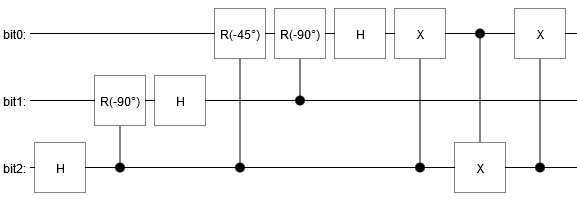
\includegraphics[width=0.8\linewidth]{qft.png}
    \caption{A circuit implementing a 3Q QFT. (Image courtesy \cite{qft})}
    \label{fig:qft}
\end{figure}

There is a well-known circuit that implements the QFT, and we show a 3Q version in fig.~\ref{fig:qft}. Once we identify that the controlled \verb|R| gates correspond to \verb|CPHASE| gates, then we can quite quickly supply the equivalent\footnote{You may notice a difference: our program uses a SWAP gate apparently not present in the original. Why do you think that is?} pyQuil program:
\begin{python}
from pyquil import Program
from pyquil.gates import *
from math import pi

qft = Program(
    SWAP(0, 2),
    H(0),
    CPHASE(-pi / 2.0, 0, 1),
    H(q1),
    CPHASE(-pi / 4.0, 0, 2),
    CPHASE(-pi / 2.0, 1, 2),
    H(2))
\end{python}

We now prepare our desired initial state. This can often be a difficult task\footnote{If you're feeling particularly peppy, have a bash at creating a $W$-state: $\tfrac{1}{\sqrt{3}}(\ket{001}+\ket{010}+\ket{100})$.}, so we'll stick to a simple initial state of $\ket{010}$
\begin{python}
initial_state = Program(I(0), X(1), I(2))
\end{python}
We need the identity gates in order to force the simulator to use three qubits. Without them, the QVM will try to optimize the program into a one-qubit one.

Almost there. Now we need a QVM to run this stuff for us. We really want access to the wavefunction amplitudes as it evolves since this is where the frequencies of the QFT will be encoded. Unfortunately this is a big no-no in quantum mechanics. Nevertheless, since we have a simulator that simulates quantum mechanics, we can pick and choose how strict we want our quantum mechanics to be: the \verb|WavefunctionSimulator| gives us enough information, and evolves the state as expected.

\begin{python}
from pyquil.api import WavefunctionSimulator

wf_sim = WavefunctionSimulator()
wf = wf_sim.wavefunction(initial_state)
print(wf)
\end{python}

$\ket{010}$ as expected. Now our program in full needs to consist of the state preparation and the QFT program

\begin{python}
prog = initial_state + qft
\end{python}

We're now ready to call out to the QVM and see where this thing takes us! Strap in.

\begin{python}
wavefunction = wf_sim.wavefunction(prog)
print(wave_function.pretty_print())
\end{python}

The result of which is 
\begin{python}
(0.35+0j)|000> + -0.35j|001> 
+ (-0.35+0j)|010> + 0.35j|011> 
+ (0.35+0j)|100> + -0.35j|101> 
+ (-0.35+0j)|110> + 0.35j|111>
\end{python}
It's not immediately obvious that this is the correct result. We can however at this point lean on the \emph{inverse} Fourier transform to confirm our hopes:

\begin{python}
from numpy.fft import ifft
wf = ifft(wavefunction.amplitudes, norm="ortho")
\end{python}

The result of which, is, again somewhat unconvincing:

\begin{python}
array([0.+0.000000e+00j, 0.+0.000000e+00j, 1.+3.061617e-17j,
       0.+0.000000e+00j, 0.+0.000000e+00j, 0.+0.000000e+00j,
       0.-3.061617e-17j, 0.+0.000000e+00j])
\end{python}

Squinting for a moment, you will notice that all but one of these entries are zero (or close enough) and we are thus left with the state $\ket{010}$. We can demonstrate that by printing the wavefunction

\begin{python}
from pyquil.wavefunction import Wavefunction
print(Wavefunction(amplitude_vector=wf)
\end{python}

\addcontentsline{toc}{section}{References}
\begin{thebibliography}{1}
  \bibitem{quilpaper} Robert S. Smith, Michael J. Curtis, William J. Zeng. {\em A Practical Quantum Instruction Set Architecture}. arXiv.org preprint. arXiv:1608.03355. 2016.
  \bibitem{noisycomp} Eric C. Peterson, Gavin E. Crooks, Robert S. Smith. {\em Fixed-Depth Two-Qubit Circuits and the Monodromy Polytope} arXiv.org preprint. arXiv:1904.10541. 2019.
  \bibitem{shouts} Robert S. Smith. {\em Someone Shouts $\ket{01000}$! Who's Excited?} arXiv.org preprint. arXiv:1711.02086. 2017.
  \bibitem{skalg} Christopher M. Dawson, Michael A. Nielson. {\em The Solovay--Kitaev Algorithm}. Quantum Information and Computation. 2005. 
  \bibitem{molmer} Klaus M{\o}lmer, Anders S{\o}rensen. {\em Multi-particle entanglement of hot trapped ions}. Physical Review Letters 82. 1999.
  \bibitem{shende} Vivek V. Shende, Igor L. Markov. {\em On the CNOT-cost of TOFFOLI gates}. Quantum Information and Computation. 2009.
  \bibitem{qft} Craig Gidney. {\it Building your own Quantum Fourier Transform}. Blog post: \url{https://algassert.com/quantum/2014/03/07/Building-your-own-Quantum-Fourier-Transform.html}. 2014. (Accessed 6 May 2019)
\end{thebibliography}

\end{document}
